\documentclass[letterpaper]{article}

\usepackage[utf8]{inputenc}
\usepackage[T1]{fontenc}
\usepackage{amsmath}
\usepackage{amssymb}
\usepackage{fancyhdr}
\usepackage{graphicx}
\graphicspath{{../figures/}}
\usepackage{subcaption}
\usepackage{tikz}
\usetikzlibrary{arrows.meta}
\definecolor{smoothblue}{HTML}{0B85A6} % S3 (docs/Style.md)
\usepackage{lastpage}
\usepackage{xcolor}

% Skeleton values to fill before submission (defined early: used in hypersetup)
\newcommand{\tok}{t\^{o}k}
\newcommand{\placeholdertitle}{TITLE TO BE FILLED}
\newcommand{\placeholdermonth}{Month 2026}

\usepackage{hyperref}
\hypersetup{
    unicode=true,
    pdftitle={tôk 1 — \placeholdertitle},
    pdfauthor={Maxime Tousignant (Smoothop)},
    pdfsubject={A publication of the tôk system},
    pdfkeywords={tok, Smoothop}
}
\usepackage{tabularx}
\usepackage{calc}
\usepackage{geometry}
\usepackage{algorithmic}
\usepackage[safe]{tipa}

% Page size and spacing
\geometry{letterpaper,left=1in, right=1in, top=1in, bottom=1in}
\setlength{\parskip}{5pt}
\setlength{\parindent}{0pt}
\raggedbottom

% Header and footer
\pagestyle{fancy}
\fancyhead[L]{Smoothop}
\fancyhead[C]{Draft --- do not distribute}
\fancyhead[R]{\placeholdermonth}
\fancyfoot[L]{}
\fancyfoot[C]{}
\fancyfoot[R]{page \thepage /\pageref*{LastPage}}

% Placeholder highlighted (to be replaced before submission)
\newcommand{\placeholder}[1]{%
  \par\smallskip\noindent
  \colorbox{yellow}{\parbox{\dimexpr\linewidth-2\fboxsep\relax}{#1}}%
  \par\smallskip}

\DeclareMathOperator*{\argmax}{arg\,max}
\DeclareMathOperator*{\argmin}{arg\,min}

% ----------------------------------------------------------------------
\begin{document}\thispagestyle{plain}
% ----------------------------------------------------------------------

\begin{center}

\includegraphics[height=1in]{smoothop_logo.pdf}

\vspace{12pt}
{\LARGE \textbf{\placeholdertitle}}

\vspace{6pt}
{\large A publication of the \tok{} system}

\vspace{12pt}
Maxime Tousignant\textsuperscript{1}

\vspace{4pt}
{\small \textsuperscript{1}\,Sustainable Development Organization Smoothop, Montreal, Canada\\
Contact: \texttt{maxime.tousignant@smoothop.org}}

\vspace{6pt}
\textit{\placeholdermonth}
\end{center}

\subsection*{Publication notice}
This document is part of the \tok{} system, an alternative economic system
developed by Smoothop (\url{https://www.smoothop.org/}). It is distributed under
the Creative Commons Attribution 4.0 International license (CC BY 4.0). The
sources of this publication --- \LaTeX{} document, figures and companion scripts
--- live at \url{https://github.com/smoothop-org/tok-system} (folder
\texttt{publications/tok\_1}).

\subsection*{AI contribution statement}
This document was prepared with the assistance of Milu, an AI agent (built on
Anthropic's Claude models) integrated into the Smoothop project. Milu's
contribution was directed and reviewed by the human author who is solely
responsible for the content of this document.

\subsection*{Abstract}
\placeholder{Abstract to be written.}

\textbf{Keywords:} \tok{} system, Smoothop.

\clearpage
% ----------------------------------------------------------------------
\section{Introduction}
% ----------------------------------------------------------------------

\placeholder{This is a skeleton document generated from the \texttt{stokex}
environment. The preamble, the Smoothop branding, the figure pipeline and the
compilation are wired and proven; the content of the tôk 1 publication remains
to be written.}

The figure below is a placeholder produced by
\texttt{figures/gen\_figures.py}, present only to prove the generation and
inclusion pipeline end to end. Replace it with the real figures.

\begin{figure}[h]
\centering
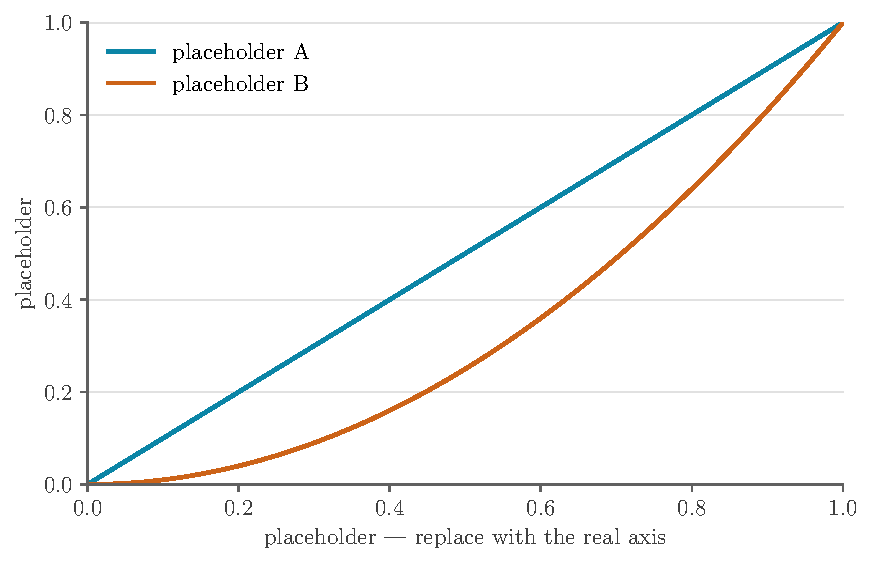
\includegraphics[width=0.75\textwidth]{tok_1_example.pdf}
\caption{Placeholder figure, in the Smoothop palette. Regenerated by
\texttt{figures/gen\_figures.py}.}
\label{figExample}
\end{figure}

% ----------------------------------------------------------------------
\section{Conclusion}
% ----------------------------------------------------------------------

\placeholder{Conclusion to be written.}

\end{document}
